\chapter{Entropy and predictability}

The potential of using a real scientific approach in order to be able to predict
where people will travel in the near or less near future can have an outstanding
impact on the way in which the engineers design and construct infrastructures
for cities, it can also impact the way in which we understand the transportation
system and, not to mention, it could give us a new insight into how we can
approach the solving of epidemics spreading \cite{Lu13} \cite{Brockmann08}.

Data from SensibleDTU \cite{Stopczynski14m} allows us to explore for research
purpose exactly how and why people move from a certain location to another. It
gives us the opportunity to look more careful into our mobility patterns in
order to try to understand how we can make use of these patterns to improve our
world.

%TODO -add no of users
In order to explore the entropy and predictability of human mobility, we have
conducted tests based on the data retrieved from a selection of users from the
SensibleDTU database. We have selected $65$ users from our original pool of
$131$ users in order to observe their movements throughout a period of $30$ days. The
reason behind discarding the remaining users was that their data was found to be
missing important fields or they did not keep their mobile phones charged and
open for the most part of the $30$ days and thus their result could have
jeopardize the study results.

\section{Entropy}

``Entropy is probably the most fundamental quantity capturing the degree of
predictability characterizing a time series'' \cite{Barabasi10}. Multiple
studies (\cite{Sinatra14},\cite{Lu13}, \cite{marin2012exploring},
\cite{Barabasi10}) that aim at understanding the predictability of the human
travel trajectory take into consideration different entropy measures which have
different meaning and different levels of importance in correctly estimating the
probability of choosing a location or another. The measures that are mentioned
are the random entropy, the temporal uncorrelated entropy, the conditional
entropy and the real entropy.

\subsection{The random entropy}
\label{r_e}

The formula for the random entropy of a random user i is given by

\begin{equation}
S_{i}^{rand} = log_{2}N_{i}
\end{equation}

Where $N_{i}$ represents the number of unique locations that
have been associated to the given user throughout the time frame that we are
taking into consideration. This measurement can be used to reflect the
predictability of the travel patterns of the given user in case we consider that
each of the locations can be visited with the exact same probability.

We have calculated the random entropy by taking into consideration the locations
visited by our selected users throughout a period of $30$ days.
Fig.~\ref{dis_r_e} shows the density distribution of the results which have been
rounded after the second decimal. As we can see, most of the users have a random
entropy of around $3.65$ and the average random entropy is $3.87$. This means
that, in average, is a user would choose randomly his or her next location, than
they can be found in any of $2^{S^{rand}} = 2^{3.87}$ locations (which is
approximately $14.62$).

\begin{figure}[!h]
\centering
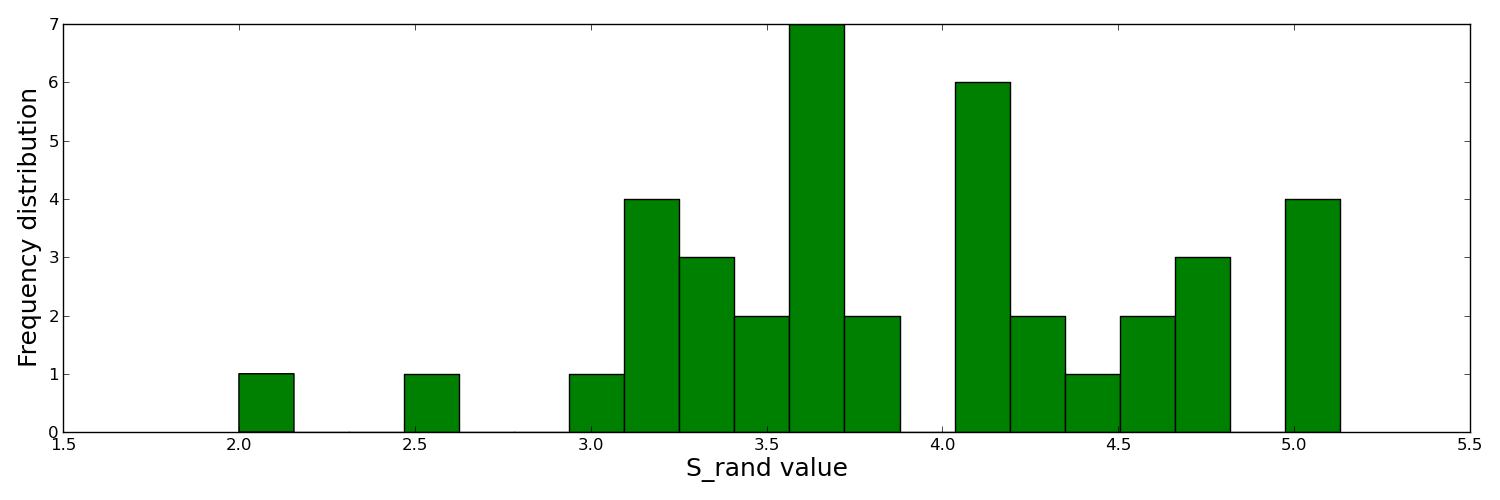
\includegraphics[width=\textwidth]{figures/entro_pred/rand_entro_distrib.png}
\caption{Density distribution for $S^{rand}$}
\label{dis_r_e}
\end{figure}

\subsection{The temporal uncorrelated entropy}
\label{tu_e}

The formula for the temporal uncorrelated entropy of a random user i is given by

\begin{equation}
S_{i}^{unc} = -\sum\limits_{j=1}^{N_{i}}p_{i}(j)log_{2}p_{i}(j)
\end{equation}

Where $N_{i}$ represents the number of unique locations that have been
associated to the given user throughout the time frame that we are taking into
consideration and $p_{i}(j)$ represents the historical probability of the given
user to visit location j. The present measurement incorporates the knowledge
about what locations occur more often in the user's traveling patterns.

We have calculated the temporal uncorrelated entropy by taking into
consideration the locations visited by our selected users throughout a period of
$30$ days. Fig.~\ref{dis_tu_e} shows the density distribution of the results
which have been rounded after the second decimal. The average temporal
uncorrelated entropy is $1.3$. This means that, in average, if we are to base
our supposition on the number of times each location has been visited in the
past by a given user, then the user's next location can be found in any of
$2^{S^{unc}} = 2^{1.3}$ locations (which is approximately $2.46$).

\begin{figure}[!h]
\centering
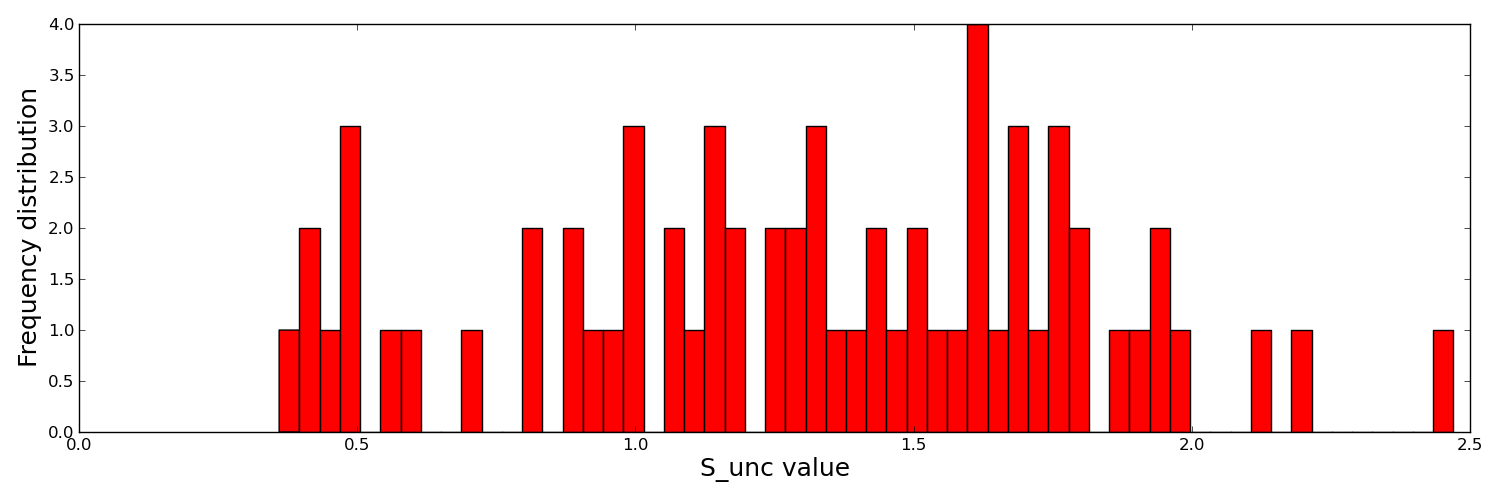
\includegraphics[width=\textwidth]{figures/entro_pred/tu_entro_distrib.png}
\caption{Density distribution for $S^{unc}$}
\label{dis_tu_e}
\end{figure}

\subsection{The conditional entropy}
\label{con_e}
The conditional entropy $S_{i}^{cond}$ for a given user $i$ is calculated based
on the formula given in the paper \cite{Sinatra14}

\begin{equation}
S_{i}^{cond} = - \sum\limits_{x_{t}\in X_{i}} \sum\limits_{x_{t-1}\in X_{i}}
p_{i}(x_{t-1},x_{t})log_{2}p_{i}(x_{t}|x_{t-1})
\end{equation}

In this formula, $x_{t}$ and $x_{t-1}$ are possible locations,
$p_{i}(x_{t-1},x_{t})$ is the probability of apparition of the subsequent
locations $x_{t-1}$ and $x_{t}$ and $p_{i}(x_{t}|x_{t-1}) = p_{i}(x_{t-1},x_{t})
/ p(x_{t-1})$ represent the probability of the user being at location $x_{t}$ at
time $t$, considering that the previous location was $x_{t-1}$. The conditional
entropy is equal to the temporal uncorrelated entropy in case we do not make any
time correlations. Also it can be proved that $S^{cond} \leq S^{unc} \leq
S^{rand}$ \cite{Cover:2006:EIT:1146355}.

In \cite{Sinatra14} the authors introduce an extension for the conditional
entropy in order to explore how the amount of previous knowledge affects the
value of the conditional entropy. The new formula is 

\begin{equation}
S_{i}^{cond,k} = - \sum\limits_{x_{t}\in X_{i}} .. \sum\limits_{x_{t-k}\in
X_{i}} p_{i}(x_{t-k},..,x_{t})log_{2}p_{i}(x_{t}|x_{t-k},..,x_{t-1})
\end{equation}

In this case, k represents the number of previous steps we know. With the
present formula it can be observed that $S_{i}^{cond,0}$ is the same with
$S_{i}^{unc}$ and that $S_{i}^{cond,1}$ is the same as $S_{i}^{cond}$.

In Fig.~\ref{conditional_e} we have the representation for the conditional
entropy calculated considering that we have knowledge of a previous time window
of $1 - 30$ time bins. It can be seen that the more information we have from the
past, the value of the conditional entropy decreases.

\begin{figure}[!h]
\centering
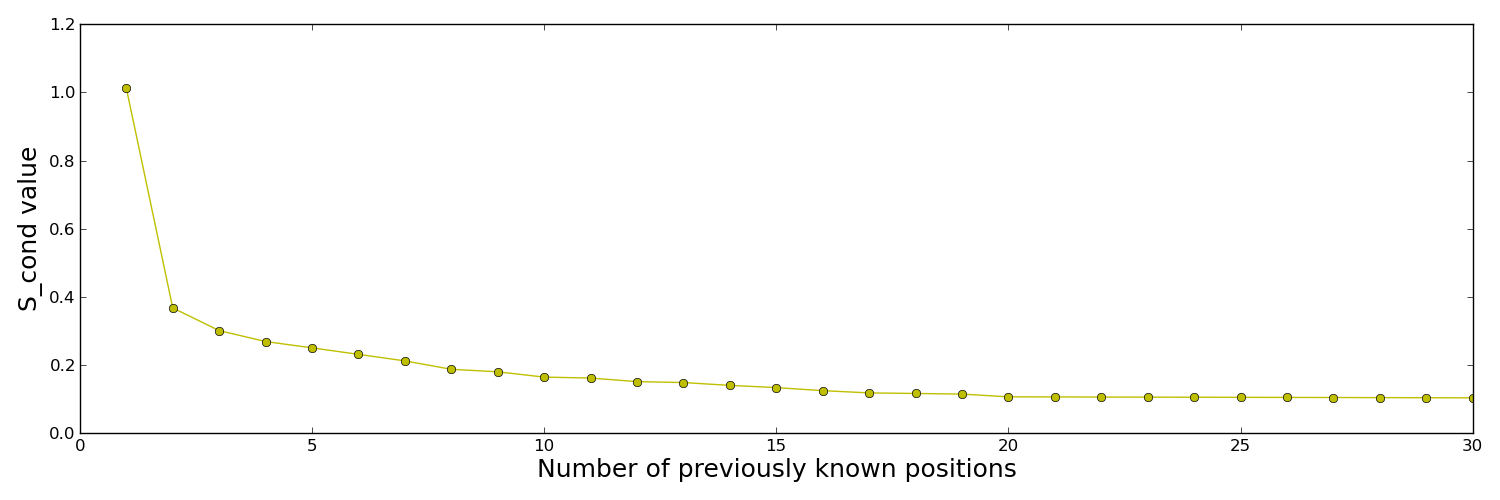
\includegraphics[width=\textwidth]{figures/entro_pred/constr.png}
\caption{$S^{cond,k}$ for a given user, where $ k \in \{1,..30\}$}
\label{conditional_e}
\end{figure}

\subsection{The real entropy}
The real entropy of a user needs to be calculated by taking into consideration
the different locations that the user has been to, the frequency with which he
or she visits these locations, the time spent at the locations and the order in
which the locations seem to follow through time. The relation between the actual
entropy and the random and time uncorrelated entropies is $S \leq S^{unc}
\leq S^{rand}$. 

If we consider that $X_{i}$ represents the locations of a user at time i,
and $h_{n}$ represents a sequence of n locations, then for a process X =
\{$X_{i}$\} the entropy can be written as
\begin{equation}
\label{eq_7_5}
S \equiv \lim_{n\to\infty} {1 \over n}S(X_{1},X_{2},..,X_{n})
\end{equation} 
\begin{equation}
\label{eq_7_6}
= \lim_{n\to\infty} \sum\limits_{i=1}^{n} S(X_{i}|h_{i-1})
\end{equation}
\begin{equation}
\label{eq_7_7}
= \lim_{n\to\infty} \sum\limits_{i=1}^{n} S(i)
\end{equation}

Equation \ref{eq_7_5} is the definition given to entropy in
\cite{Cover:2006:EIT:1146355}, equation \ref{eq_7_6} reflects the application of
the chain rule in the previous equation and $S(X_{i}|h_{i-1})$ represents the
conditional entropy at step n in equation \ref{eq_7_7} \cite{song2010limits}.

The paper \cite{Barabasi10} present another way in which the entropy for a user
i can be written. If we consider that $T_{i} = {X_{1}, X_{2},\ldots, X_{n}}$
represents the sequence of locations which have been visited by user i and if we
consider that $P(T'_{i})$ represents the probability of finding time ordered
subsequence $T'_{i}$ in the trajectory $T_{i}$, then the entropy of user i can
be written as

\begin{equation}
S_{i} = - \sum\limits_{T'_{i}\subset T_{i}}P(T'_{i})log_{2}[P(T'_{i})]
\end{equation}

We have calculated a measurement of the entropy for our selected users and the
distribution for the results which have been rounded after the second decimal
can be seen in Fig.~\ref{dis_full_e}. The fact that the average value of the
real entropy for the selected user is around $0.17$ means that, in reality we
the uncertainty about where a user will be traveling to next is $2^{0.17} =
1.12$ locations. These findings show that, the users we have been observing do
not randomly choose their future locations, but in fact, their locations are
well established by restrictions such as hours or days at which they need to be
at work, or school as well as other patterns that govern most of the times our
decisions.

\begin{figure}[!h]
\centering
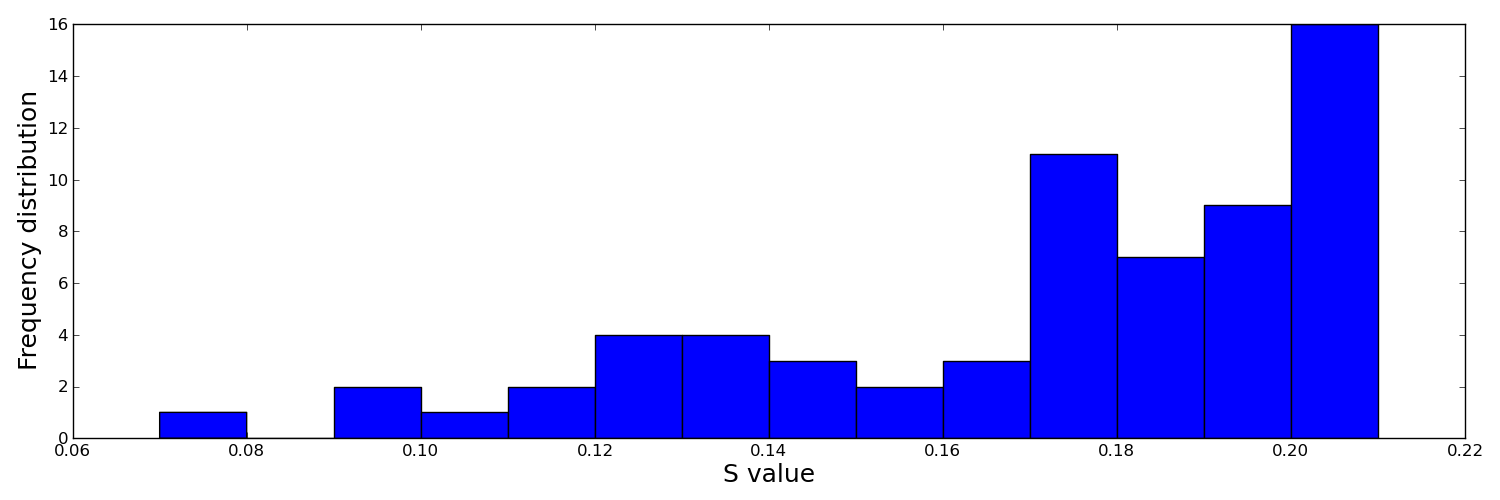
\includegraphics[width=\textwidth]{figures/entro_pred/full_entro_distrib.png}
\caption{Density distribution for $S$}
\label{dis_full_e}
\end{figure}

In Fig.~\ref{dis_overlay} we have an overlay of the distribution for the random,
temporal uncorrelated and real entropies.

\begin{figure}[!h]
\centering
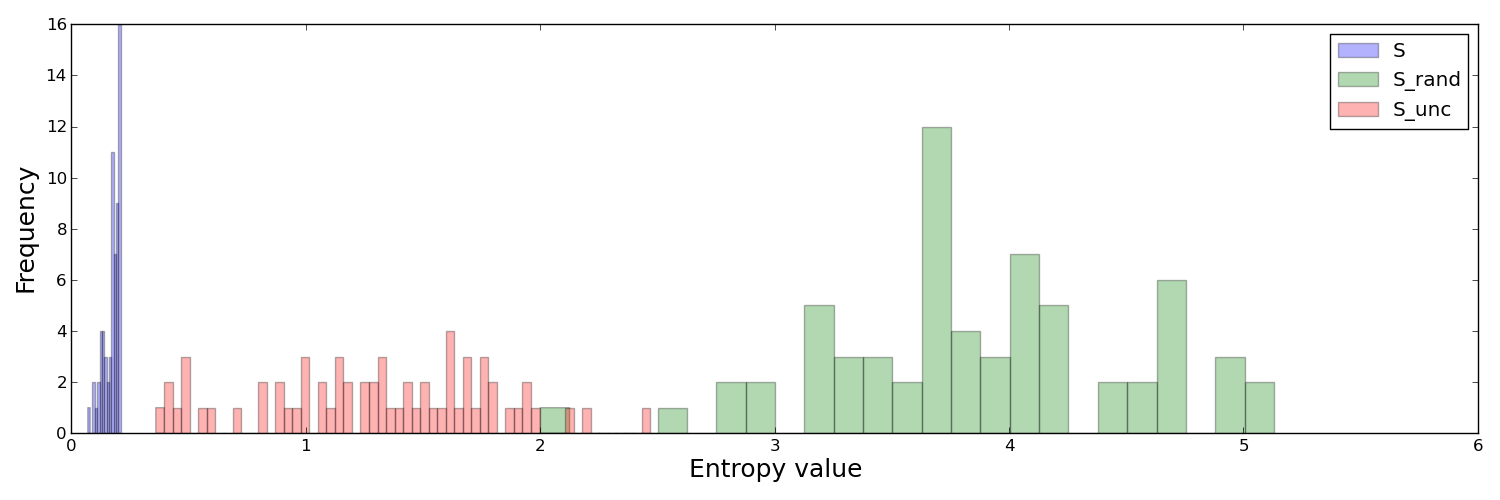
\includegraphics[width=\textwidth]{figures/entro_pred/overlay.png}
\caption{Density distributions for $S$, $S^{rand}$ and $S^{unc}$}
\label{dis_overlay}
\end{figure}

\section{Predictability}

A measure that needs to be taken into consideration when discussing
predictability is the probability ($\Pi$) of a predictive algorithm to correctly
estimate the future locations a user will visit. According to the inequality of
Fano \cite{brabazon2008natural} \cite{1057678}, a user for which the entropy is
S and it has been calculated taking into consideration the fact that the user
spends his or her time in either of N given locations, then his or her
predictability (as it is presented in \cite{Barabasi10} and in \cite{Sinatra14}
as well) is given by

\begin{equation}
\label{ineq_pred}
\Pi \leq \Pi^{max}(S,N)
\end{equation}

The value for $\Pi^{max}$ can be determined from

\begin{equation}
\label{pred}
S = H(\Pi^{max}) + (1 - \Pi^{max})log_{2}(N-1)  
\end{equation}

by knowing that

\begin{equation}
\label{h_func}
H(\Pi^{max}) = - \Pi^{max}log_{2}(\Pi^{max}) - (1-\Pi^{max})log_{2}(1-\Pi^{max})   
\end{equation}  

By combining the two previous formula we obtain the equation

\begin{equation}
\label{equation}
S + \Pi^{max}log_{2}(\Pi^{max}) + (1-\Pi^{max})log_{2}(1-\Pi^{max}) - (1 -
\Pi^{max})log_{2}(N-1) = 0
\end{equation}

One of the aims of our study is to estimate the predictability when it comes to
the trajectory patterns of the selected users from the SensibleDTU database.
After we have calculated their entropy and after knowing the number of locations
each of them has been traveling in between for the duration of $30$ days that we
considered for our experiment, we only needed to calculate the entropy based on
the mathematical formulae at \ref{pred} and \ref{h_func}. However, the equation
at \ref{equation}, which would allow us to calculate the predictability for each
user is a transcendent equation. This means that the equation can be solved
either numerically or graphically.

In order to solve the equation we use a numerical method that helped us
approximate the result. The method we use is the bisection method \cite{faires}.
This method is applicable for solving an equation $f(x) = 0$ over a given
interval $[a,b]$ for which the values $f(a)$ and $f(b)$ have opposing sings. In
our case the f function is represented by the left side in the equation
\ref{equation}. Since the solution of our equation $f(x) = 0$ needs to be a
number between 0 and 1 (the maximum predictability can only have a value in this
interval), than we start the algorithm by verifying if by replacing the maximum
predictability with 0 or 1 we have a solution or if the two values obtained this
way have opposing signs. If they have opposing signs, we consider that $a = 0$
and $b = 1$. In case the function does not have opposing signs, we adjust the
interval until we find either a solution or values for which the signs are
opposing. The algorithm continues as following:
\begin{itemize}
  \item As long as we do not exceed a previously set number of iterations we
  look for the middle of the interval given by the selected a and b numbers
  (let the middle be m)
  \item In case $f(m)$ is 0 or sufficiently close to 0 (we accept an error of
  order $10^{-3}$), than we have found our solution, otherwise if the value of
  $f(m)$ has the same sign as $f(a)$ we move forward considering the interval
  $[m,b]$, if it has the same sign as $f(b)$ we continue by using the interval
  $[a,m]$
  \item We increment the number of iterations we have computed
\end{itemize}

The average predictability value for the selected users and through the given
$30$ days of observations is of approximately $98\%$ which supports the
observations made in previous studies (a considerable number of which have
already been mentioned in the present paper - e.g. \cite{song2010limits},
\cite{Barabasi08} etc) regarding the fact that we seem to have a highly well
established pattern of traveling that rises from our daily habits.

% 6 pages \begin{enumerate} \item Calculating entropy for users \item
% Calculating predictability for users \item Observations end{enumerate}
